\documentclass[a4paper,10pt,hidelinks]{scrartcl}

% packages
\usepackage[ngerman]{babel}
\usepackage{graphicx}
\usepackage{hyperref}
\usepackage{url}
\usepackage{fontspec}
    \setmainfont{Arial}
    \setsansfont{Arial}
    \setmonofont{Inconsolata}
\usepackage{fancyhdr}
\usepackage[paper=a4paper,left=20mm,right=20mm,top=40mm,bottom=25mm,headheight=40mm]{geometry}
\usepackage{tabto}
\usepackage{sectsty}
\usepackage{afterpage}
\usepackage{listings}
\usepackage{blindtext}

% global options
\renewcommand{\baselinestretch}{1.25}

\lstset{basicstyle=\small\ttfamily,captionpos=b,xleftmargin=0.25in,xrightmargin=0.25in}

% header/footer
\pagestyle{fancy}
\renewcommand{\headrulewidth}{0pt}
\renewcommand{\footrulewidth}{0pt}
\rhead{
\includegraphics[width=40mm]{pics/header-2.png}}
\rfoot{
\includegraphics[width=40mm]{pics/footer.png}}
\fancypagestyle{firstpage}{
    \rhead{
\includegraphics[width=40mm]{pics/header-1.png}}
}
\cfoot{}

\newcommand{\imgref}[1]{{Abbildung \ref{#1}, Seite \pageref{#1}}}

\begin{document}

\section*{\fontsize{18}{20}\selectfont Enterprise Lab Storage}
\thispagestyle{firstpage}

\textbf{Themenbereiche:} \tabto{4cm} Erneuerung Storage im Enterprise Lab

\noindent
\textbf{Studierender:} \tabto{4cm} Einfalt S. Pinsel

\noindent
\textbf{Betreuungsperson:} \tabto{4cm} Juno Broho

\noindent
\textbf{Experte:} \tabto{4cm} Prof. Dr. phil. nat. Markus Christ

\noindent
\textbf{Auftraggebende:} \tabto{4cm} Dr. Hans Dampf

\noindent
\textbf{Keywords:} \tabto{4cm} Enterprise Lab, Storage Array, höhere Cyberkunde

\section{\fontsize{14}{16}\selectfont Aufgabenstellung}

\Blindtext

Die bestehende Storage-Lösung des Enterprise Labs ist in \imgref{fig:storage-old} dargestellt.

\begin{figure}
    \centering
    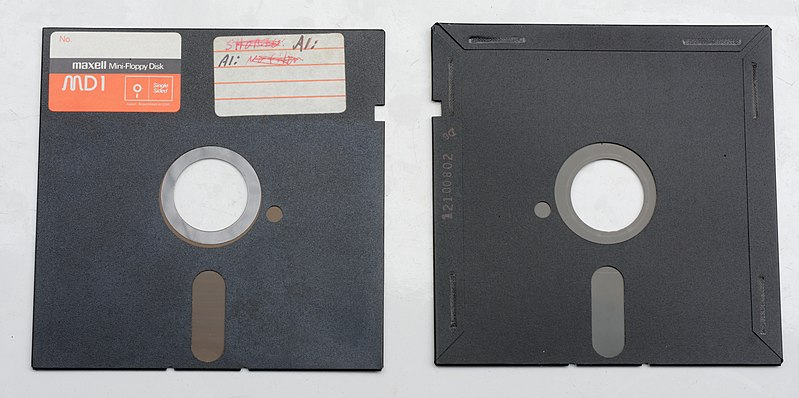
\includegraphics[width=0.5\linewidth]{pics/storage-old.jpg}
    \caption{Die bestehende Storage-Lösung im Enterprise Lab}
    \label{fig:storage-old}
\end{figure}

\section{\fontsize{14}{16}\selectfont Ergebnisse}

\blindtext

Die Einrichtung der Storage-Medien:

\begin{lstlisting}
C:> format A:\
WARNING, ALL DATA ON NON-REMOVABLE DISK
Drive A: WILL BE LOST!
Proceed with Format (Y/N)?
\end{lstlisting}

\blindtext

\section{\fontsize{14}{16}\selectfont Lösungskonzept}

\blindtext

\begin{figure}
    \centering
    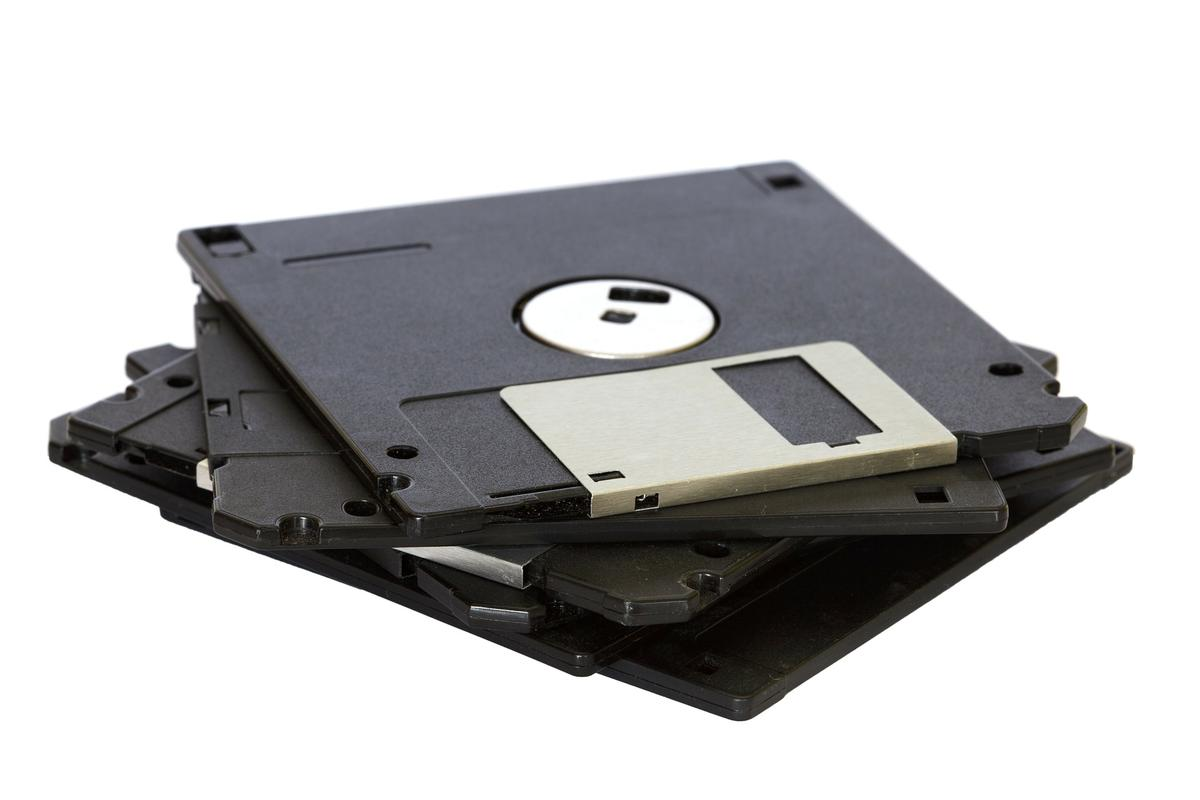
\includegraphics[width=0.4\linewidth]{pics/storage-new.jpg}
    \caption{Die Storage-Lösung für das nächste Jahrtausend}
    \label{fig:storage-new}
\end{figure}

Die erneuerte Storage-Lösung des Enterprise Labs ist in \imgref{fig:storage-new} dargestellt.

\section{\fontsize{14}{16}\selectfont Spezielle Herausforderungen}

\blindtext

\section{\fontsize{14}{16}\selectfont Ausblick}

\blindtext

\end{document}
